% coding:utf-8

\section{Aufgabe 1}

\subsection{a}
\begin{Schunk}
\begin{Sinput}
> # forbes <- read.table("http://stat.ethz.ch/Teaching/Datasets/forbes.dat",header=TRUE)
> forbes <- read.table("forbes.dat",header=TRUE)
> plot(forbes[,"Temp"], forbes[,"Press"])
\end{Sinput}
\end{Schunk}
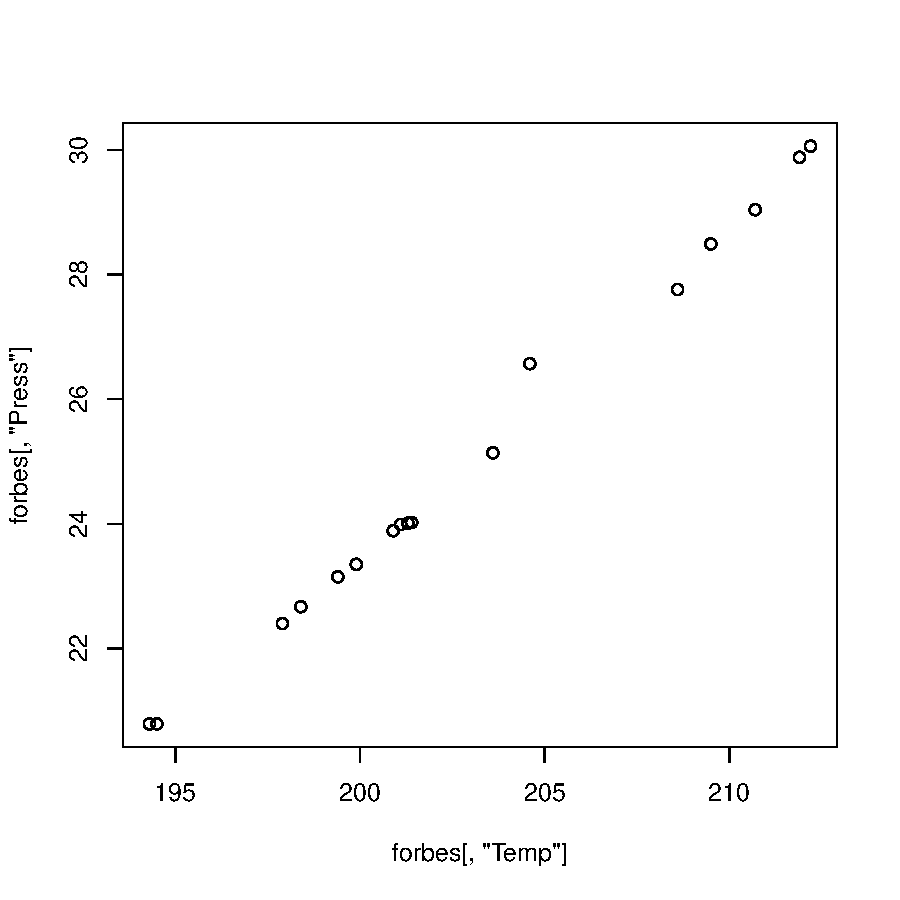
\includegraphics{sw12_1-001}

\subsection{b}
\begin{Schunk}
\begin{Sinput}
> forbes.fit <- lm(Press ~ Temp, data = forbes)
> summary(forbes.fit)
\end{Sinput}
\begin{Soutput}
Call:
lm(formula = Press ~ Temp, data = forbes)

Residuals:
     Min       1Q   Median       3Q      Max 
-0.25717 -0.11246 -0.05102  0.14283  0.64994 

Coefficients:
             Estimate Std. Error t value Pr(>|t|)    
(Intercept) -81.06373    2.05182  -39.51   <2e-16 ***
Temp          0.52289    0.01011   51.74   <2e-16 ***
---
Signif. codes:  0 ‘***’ 0.001 ‘**’ 0.01 ‘*’ 0.05 ‘.’ 0.1 ‘ ’ 1 

Residual standard error: 0.2328 on 15 degrees of freedom
Multiple R-squared: 0.9944,	Adjusted R-squared: 0.9941 
F-statistic:  2677 on 1 and 15 DF,  p-value: < 2.2e-16 
\end{Soutput}
\begin{Sinput}
> plot(forbes[,"Temp"], forbes[,"Press"])
> abline(forbes.fit)
\end{Sinput}
\end{Schunk}
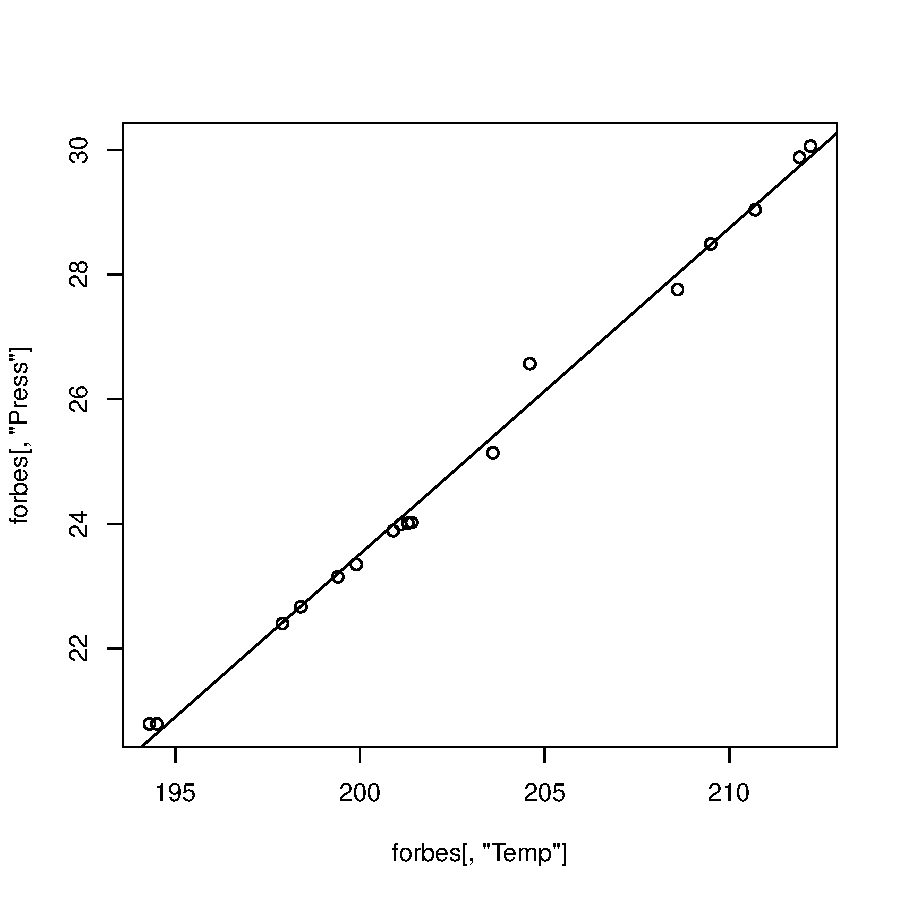
\includegraphics{sw12_1-002}

\subsection{c}
\begin{Schunk}
\begin{Sinput}
> plot(fitted(forbes.fit), resid(forbes.fit), main="Tukey-Anscombe Plot")
> abline(h=0)
\end{Sinput}
\end{Schunk}
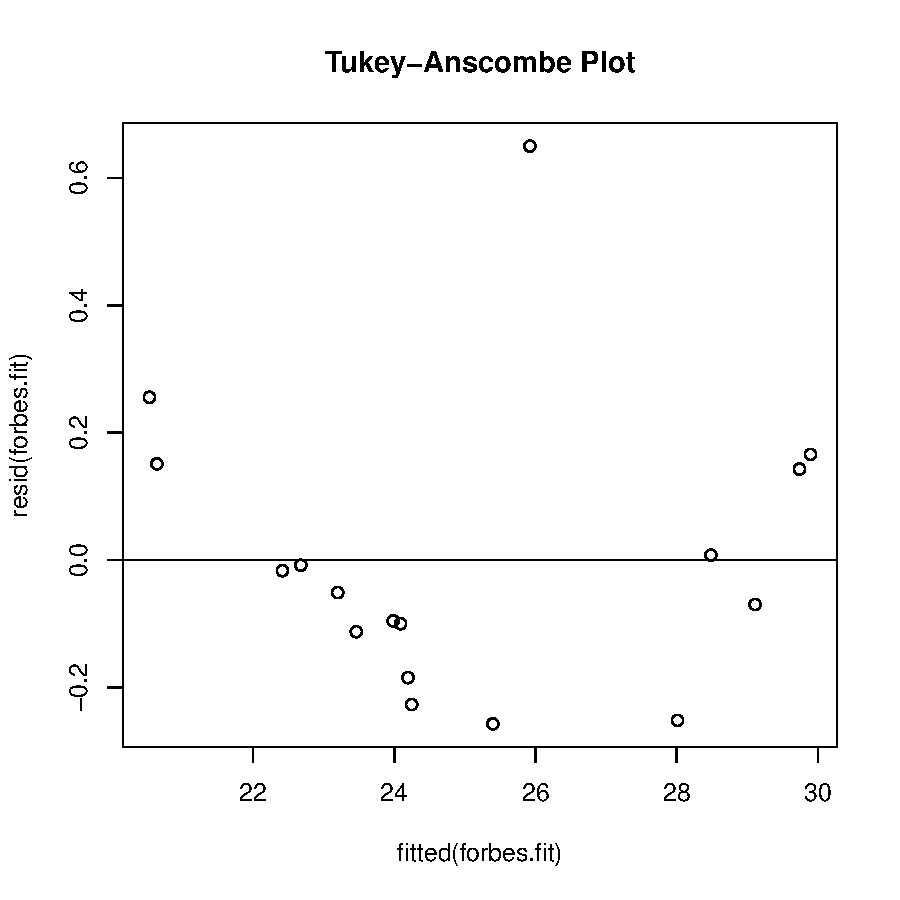
\includegraphics{sw12_1-003}
\begin{Schunk}
\begin{Sinput}
> qqnorm(resid(forbes.fit))
> qqline(resid(forbes.fit))
\end{Sinput}
\end{Schunk}
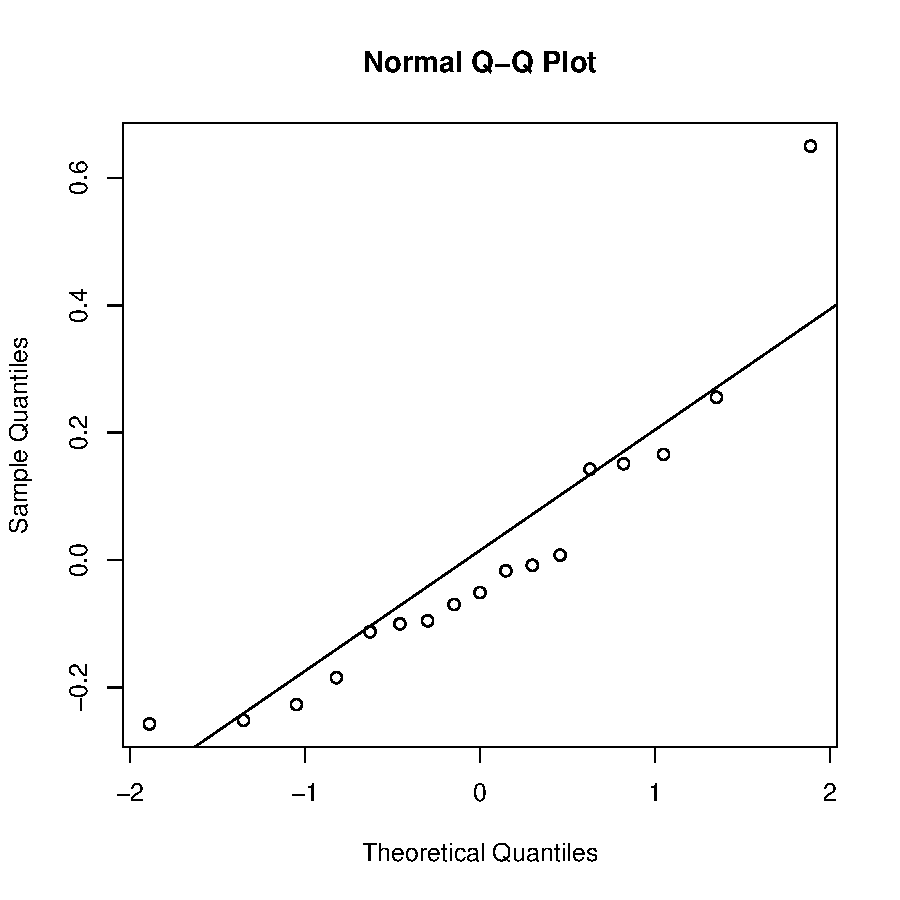
\includegraphics{sw12_1-004}

\subsection{d}
\begin{Schunk}
\begin{Sinput}
> forbes[,"Logpress"] <- log(forbes[,"Press"])
> plot(forbes[,"Temp"], forbes[,"Logpress"])
> forbes.log.fit <- lm(Logpress ~ Temp, data = forbes)
> abline(forbes.log.fit)
\end{Sinput}
\end{Schunk}
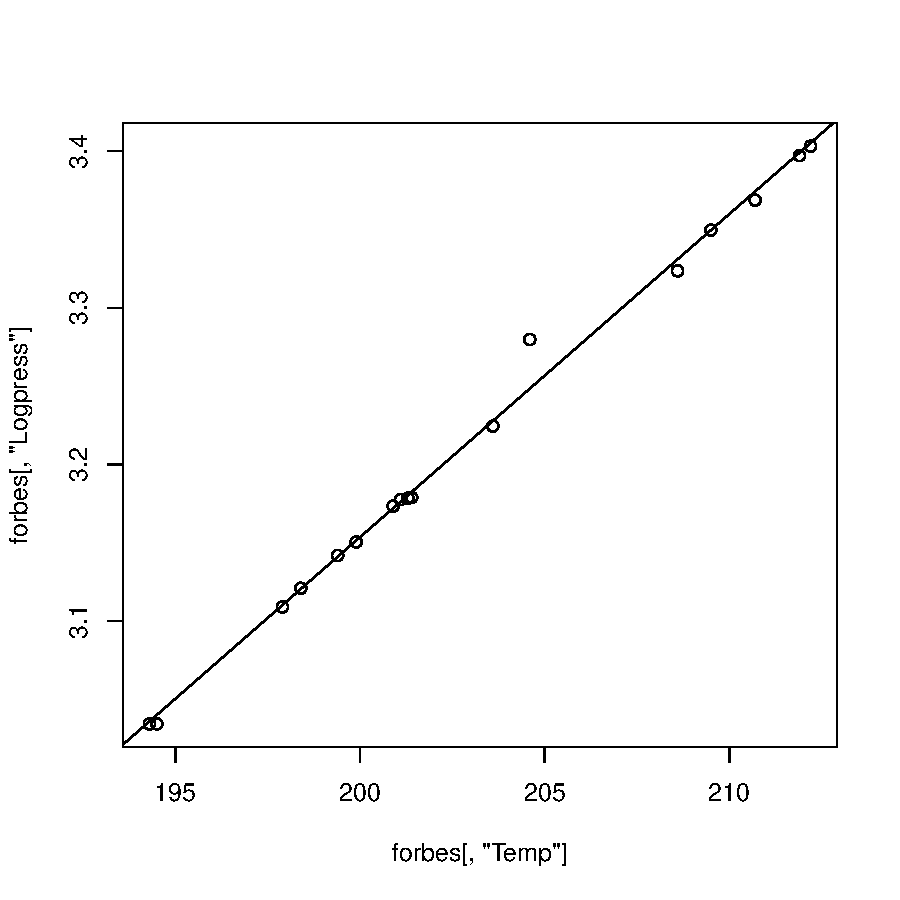
\includegraphics{sw12_1-005}

\subsection{e}
\begin{Schunk}
\begin{Sinput}
> plot(fitted(forbes.log.fit), resid(forbes.log.fit), main="Tukey-Anscombe Plot")
> abline(h=0)
\end{Sinput}
\end{Schunk}
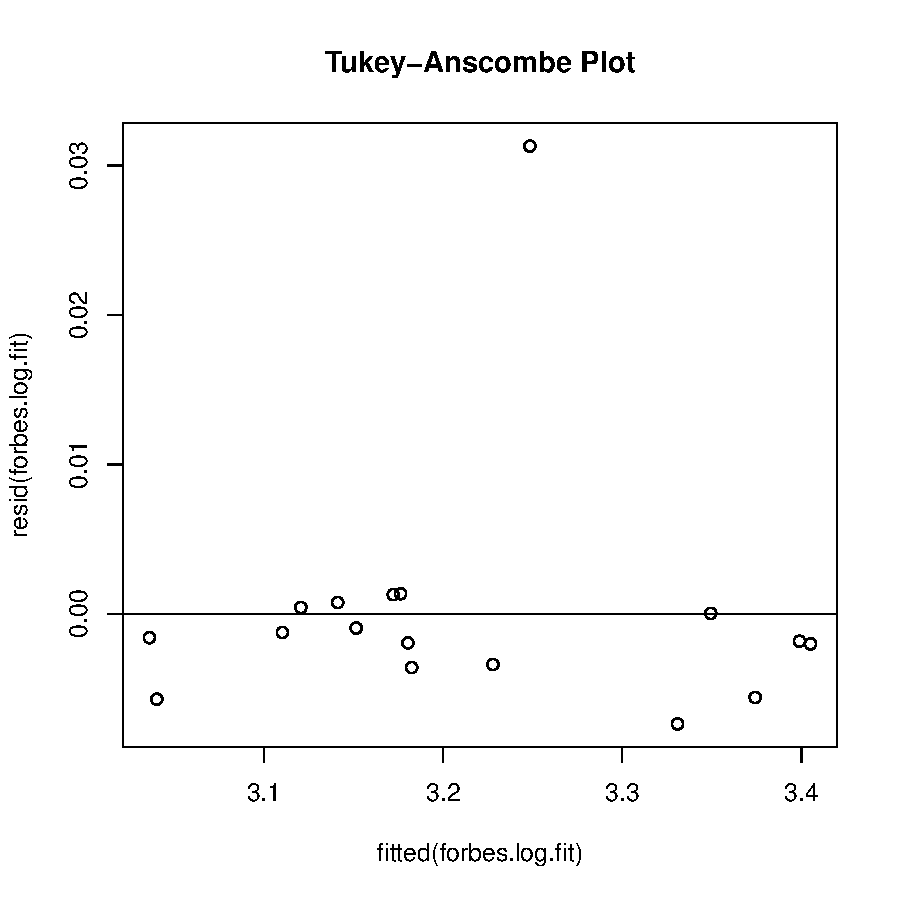
\includegraphics{sw12_1-006}
\begin{Schunk}
\begin{Sinput}
> qqnorm(resid(forbes.log.fit))
> qqline(resid(forbes.log.fit))
\end{Sinput}
\end{Schunk}
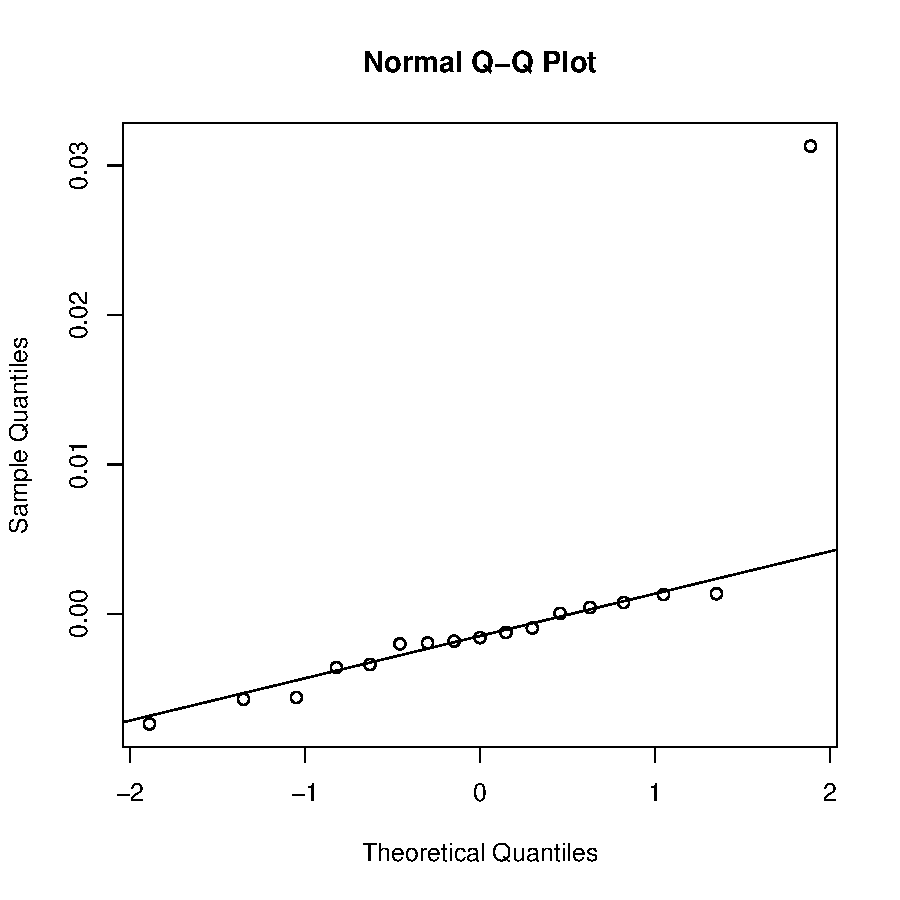
\includegraphics{sw12_1-007}

\subsection{f}
\begin{Schunk}
\begin{Sinput}
> plot(fitted(forbes.log.fit), resid(forbes.log.fit), main="Tukey-Anscombe Plot")
> abline(h=0)
> # identify(fitted(forbes.log.fit), resid(forbes.log.fit))
> forbes.korr=forbes[-12]
\end{Sinput}
\end{Schunk}
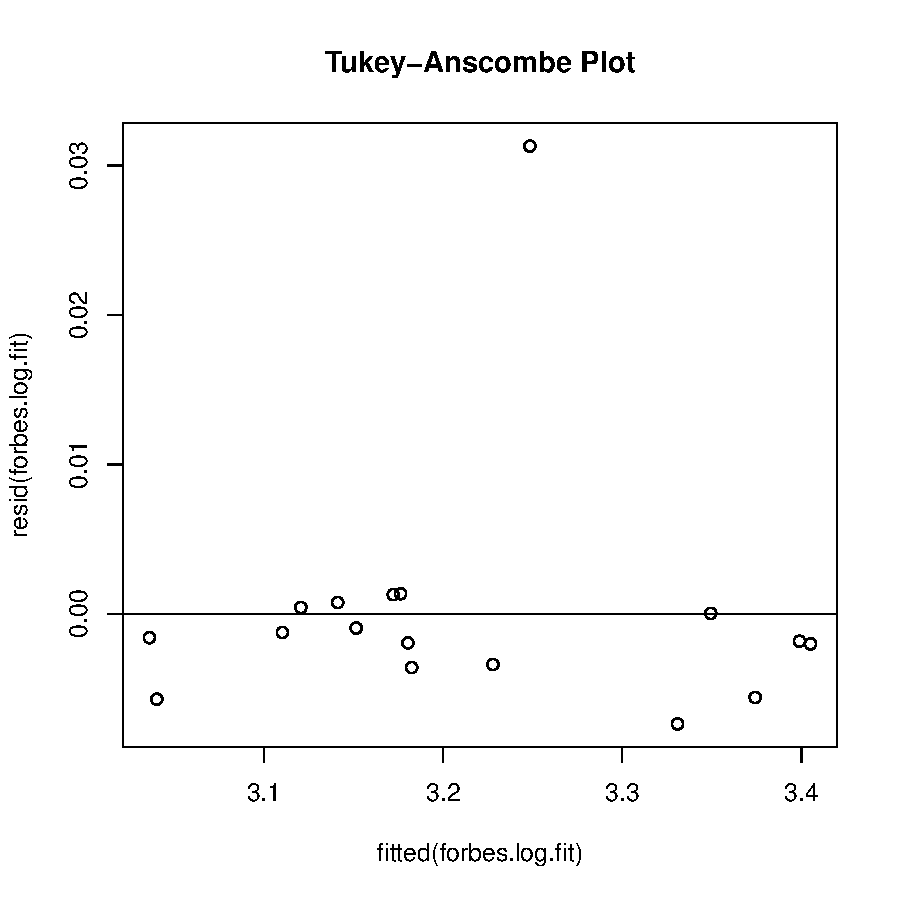
\includegraphics{sw12_1-008}
\begin{Schunk}
\begin{Sinput}
> forbes.korr.fit <- lm(Press ~ Temp, data = forbes.korr)
> # summary(forbes.korr.fit)
> plot(forbes.korr[,"Temp"], forbes.korr[,"Press"])
> abline(forbes.korr.fit)
\end{Sinput}
\end{Schunk}
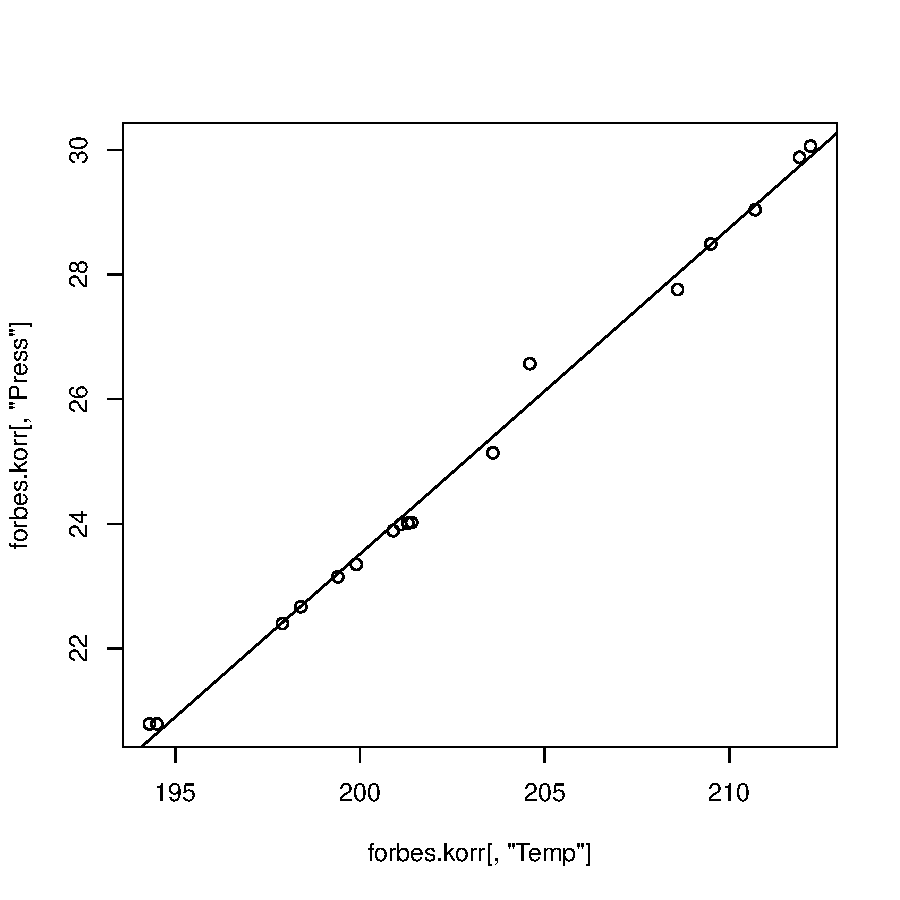
\includegraphics{sw12_1-009}
\begin{Schunk}
\begin{Sinput}
> plot(fitted(forbes.korr.fit), resid(forbes.korr.fit), main="Tukey-Anscombe Plot")
> abline(h=0)
\end{Sinput}
\end{Schunk}
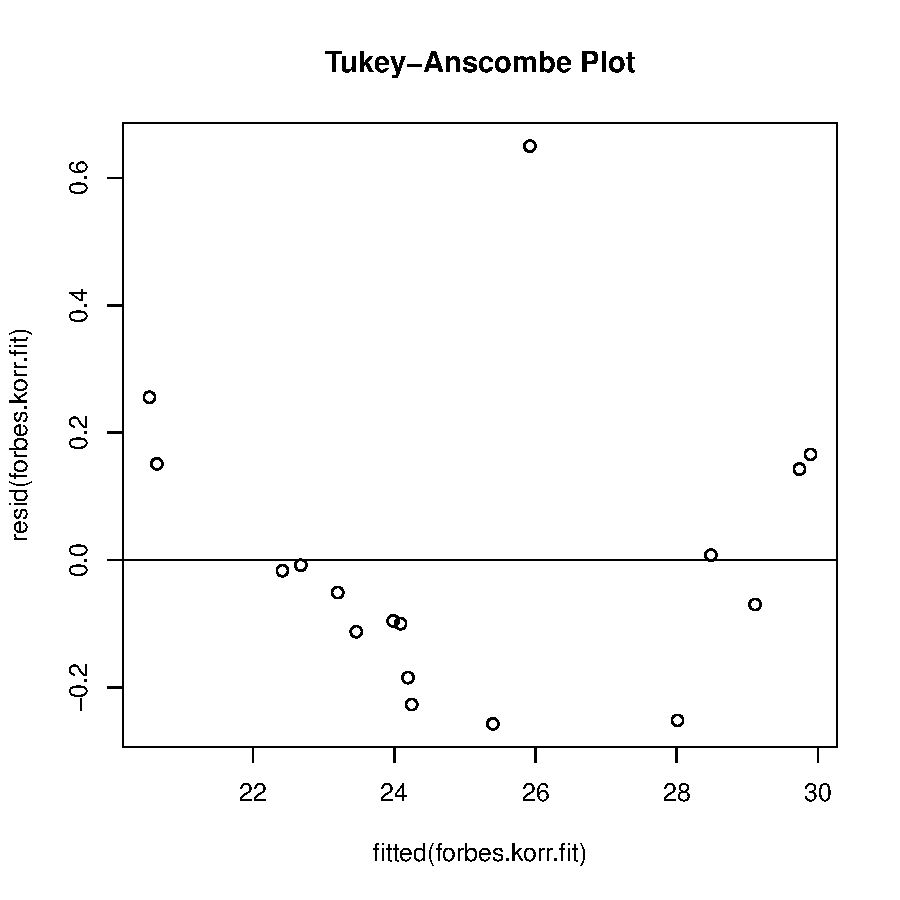
\includegraphics{sw12_1-010}
\begin{Schunk}
\begin{Sinput}
> qqnorm(resid(forbes.korr.fit))
> qqline(resid(forbes.korr.fit))
\end{Sinput}
\end{Schunk}
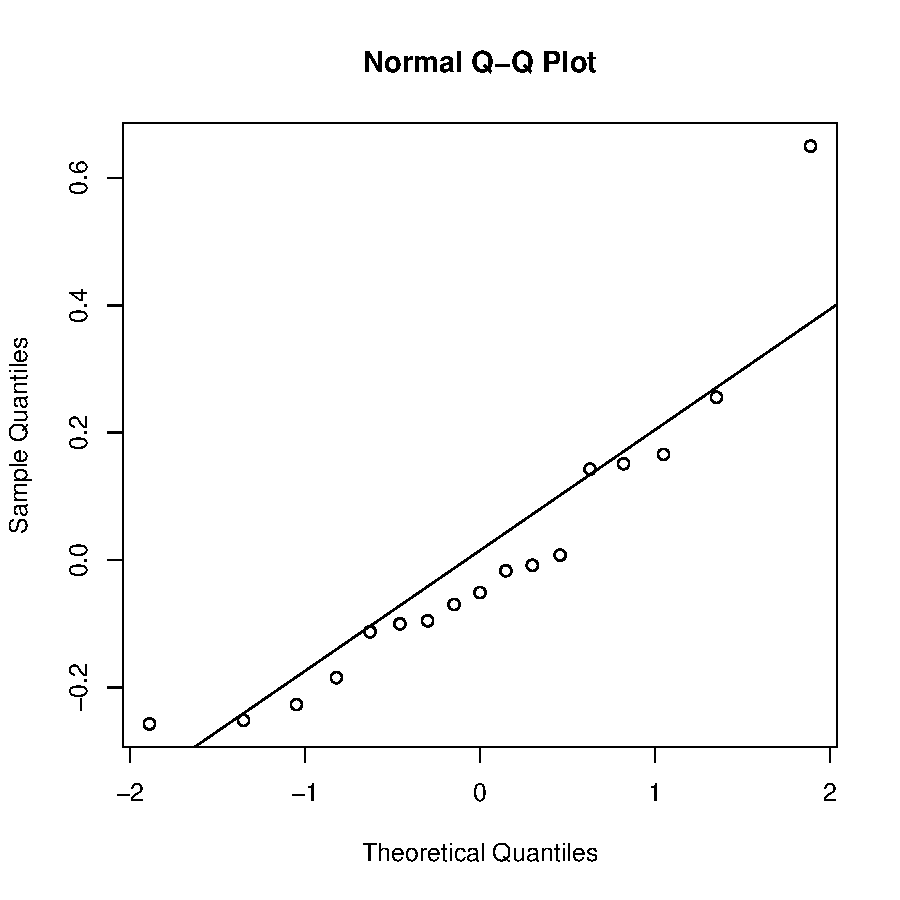
\includegraphics{sw12_1-011}
\begin{Schunk}
\begin{Sinput}
> forbes.korr[,"Logpress"] <- log(forbes.korr[,"Press"])
> plot(forbes.korr[,"Temp"], forbes.korr[,"Logpress"])
> forbes.korr.log.fit <- lm(Logpress ~ Temp, data = forbes.korr)
> abline(forbes.korr.log.fit)
\end{Sinput}
\end{Schunk}
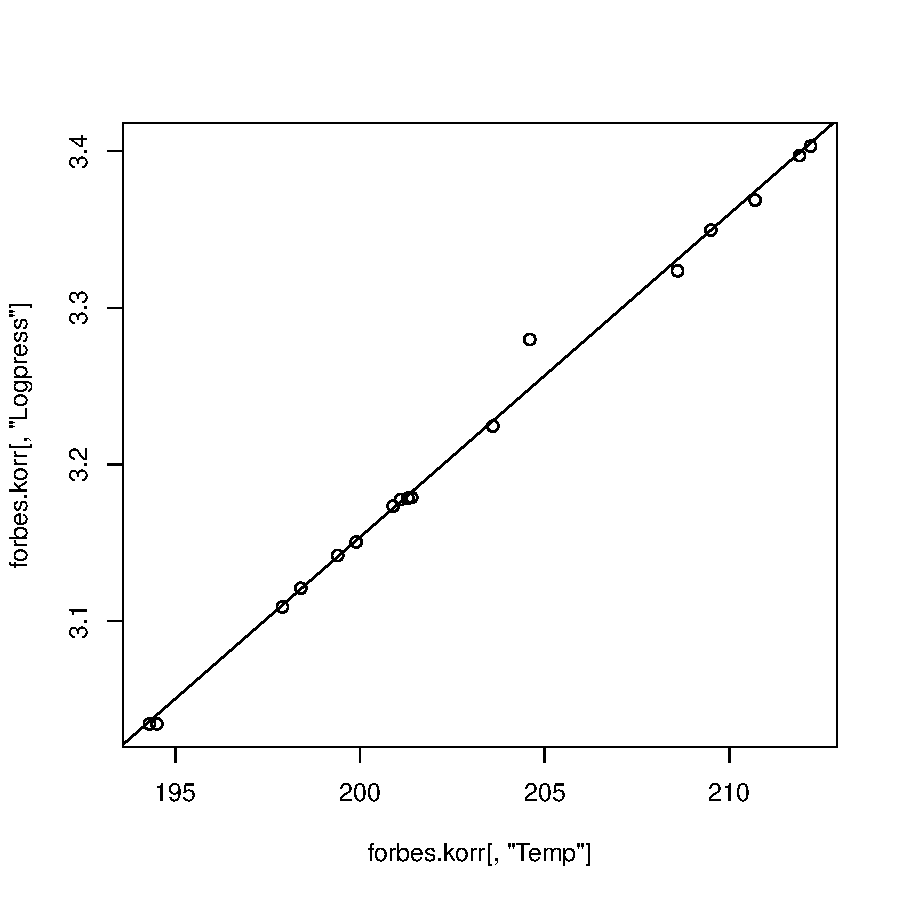
\includegraphics{sw12_1-012}
\begin{Schunk}
\begin{Sinput}
> plot(fitted(forbes.korr.log.fit), resid(forbes.korr.log.fit), main="Tukey-Anscombe Plot")
> abline(h=0)
\end{Sinput}
\end{Schunk}
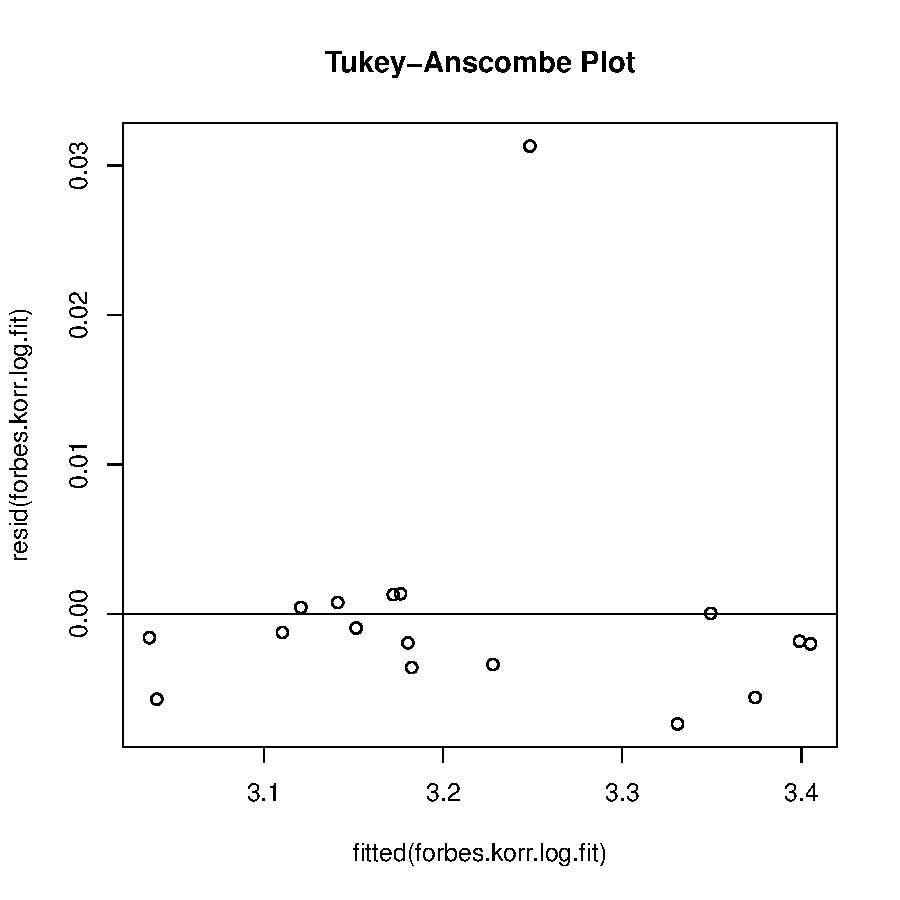
\includegraphics{sw12_1-013}
\begin{Schunk}
\begin{Sinput}
> qqnorm(resid(forbes.korr.log.fit))
> qqline(resid(forbes.korr.log.fit))
\end{Sinput}
\end{Schunk}
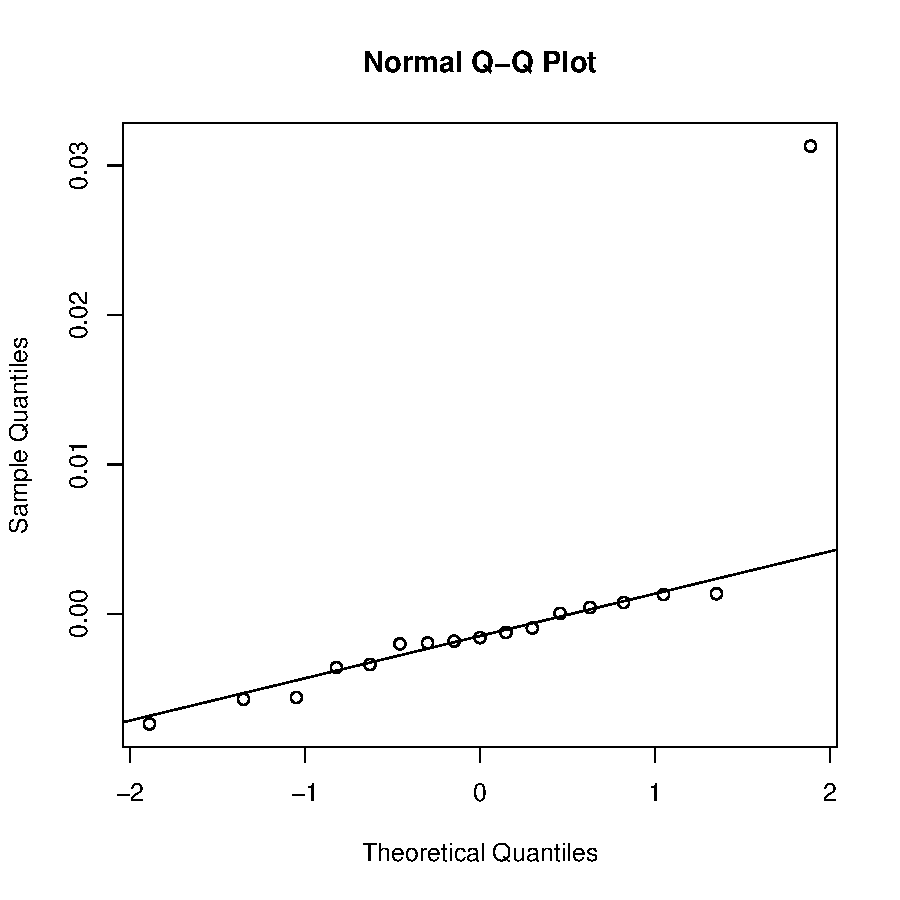
\includegraphics{sw12_1-014}
